\chapter{Testovanie}\label{test}
Testovanie prebiehalo v dvoch prostrediach. 
Jedným bolo simulované prostredie, ktorého zameraním bolo overiť funkciu algoritmu a logiky ovládania inteligentného vykurovania. Opísané v podkapitole \ref{test-sim}.
Druhým prostredím bolo réalne prostredie, teda konkrétna miestnosť ovládaná inteligentným vykurovaním. 
Proces tohto testovania, jeho detaily a výsledky sú opísané v podkapitole \ref{test-real}.

\section{Testovanie v simulovanom prostredí}\label{test-sim}
Toto prostredie bolo vytvorené nad implementovaným algoritmom. 
Implementáciu simulácie je možné najsť na stránkach \emph{GitHub\footnote{Konkrétny link je \url{https://github.com/Siki-ux/bp-int-heating/tree/main/test_algo}.}.}
Ten bol napojený na fiktívnu datábazu reprezentovanú statickými údajmi. 
Hlavnou čásťou simulácie bol cyklus reprezentujúci cyklickú obsluhu s intervalom 5 minút. 
Vývoj teploty prostredia bol simulovaný pseudonáhodnými číslami, ktoré predstavovali pohyb teploty.
To znamená, že teplota v miestnosti klesá o náhodnú teplotu, z limitu každý cyklus, pričom vzácne môže teplota aj stúpnuť.
Tento pohyb bol ďalej modifikovaný do tvaru goniometrické sinusoidy s periódou 24 posunutou o 8 hodín.
To s cieľom simulovať priebeh teploty počas dňa.
V simulácii bolo možné nastaviť všetky podstatné premenné inteligentného vykurovania, počiatočné body simulácie a koeficienty vyhrievania, chladenia a goniometrickej funkcie.
Dva simulované senzory \emph{RisingHF1S001}, opísané v podkapitole \ref{impl-Rising}, odosielali teplotu do simulovanej databáze každý cyklus.
Po zavedení simulovaného regulátoru \emph{Vicki}, opísaného v podkapitole \ref{impl-Vicki}, je stúpavý pohyb teploty navýšený o výkon výhrevného telesa.
Regulácia, teda pohyb motora, čo má za následok zvýšenie alebo zníženie výkonu výhrevného telesa, je vypočítavaná v rovnakom cykle.
Výstupom simulácie je tabuľka meraných veličín, ktorá bola väčšinou vizualizovaná na grafe v programe \emph{MS Excel}.

Počas testovania bolo otestovaných niekoľko systémov ovládania regulácie vykurovania. 
Patril medzi ne aj robustný \emph{PID systém}, ktorý však nebolo možné efektívne implementovať do riešenia \emph{iTemp} a zároveň jeho výsledky, aj napriek rozsiahlemu testovaniu s rôznymi vstupmi, nepreukázali požadované výsledky.
Zapríčinené to mohlo byť aj nie najlepším návrhom simulovaného prostredia.
Najideálnejšie výsledky v širšom časovom pásme preukázal pôvodne navrhovaný algoritmus opísaný v podkapitole \ref{navrh-algo}.

Na obrázku \ref{fig:simGraph}, je možné vidieť výstup jedneho z testov. 
Tento test začínal na počiatočnej teplote 20°C v 48 hodinách. 
Násobok úbytku teploty bol 1 a vyhrievania bol 8. 
Algoritmus používal koeficient 5. 
Na základe grafu je možné vidieť, že algoritmus splnil požiadavky aby maximálny rozdiel nameranej a požadovanej teploty bol 1°C a použil k tomu malý počet pohybov motora. 
Algoritmus čiastočne sinusoidu vyrovnal, čo sa dá porovnať s obrázkom \ref{fig:simGraphNoHeating}, kde je vyobrazený priebeh bez spusteného vykurovania.

\begin{figure}[H]
    \centering
    \includesvg[inkscapelatex=false,width=0.9\textwidth]{obrazky-figures/simGraph.svg}
    \caption{Graf teplôt a pozície motora v simulácii.}
    \label{fig:simGraph}
\end{figure}

\begin{figure}[H]
    \centering
    \includesvg[inkscapelatex=false,width=0.9\textwidth]{obrazky-figures/simGraphNoHeating.svg}
    \caption{Graf vývoja teploty v simulácii.}
    \label{fig:simGraphNoHeating}
\end{figure}



\section{Testovanie v reálnom prostredí}\label{test-real}
Toto testovanie prebiehalo v jednej miestnosti bytu vo vežiaku. 
Testovacie prostredie, teda miestnosť bola o rozlohe $12.2 m^2$ s jedným výhrevným telesom. 
Tým bol liatinový radiátor, napojený na ustredný zdroj tepla. 
Na ventil radiátora bola napojená inteligentná hlavica \emph{Vicki} opísaná v podkapitole \ref{impl-Vicki}. 
Nad radiátorom sa nachádzalo plastové dvojokno. 
Dvere miestnosti boli situované do uzavretého priestoru a nachádzali sa naoproti oknu s radiátorom. 
Na účeli testovania boli použité dva tepelné senzory \emph{RisingHF1S001} opísané v podkapitole \ref{impl-Rising}. 
Prvý bol umiestnený v blízkosti okna a radiátora a druhý bol umiestnený približne v strede miestnosti vo výške $1.2 m$.
Všetky tri zariadenia spadali pod rovnaký systém a boli umiestnené do rovnakej skupiny, teda miestnosti.
Koeficient miestnosti bol nastavený na 3.
Zariadenia monitorujúce a ovládajúce teplotu v miestnosti sú odfotené na~obrázkoch \ref{fig:test_device}.

Po spustení zariadení a nastavení požadovanej teploty aplikáciou \emph{iTemp} podľa obrázka~\ref{fig:test_setTarget}, začala rutina ovládať túto miestnosť. 
To sa postupne prejavilo na štatistikách zariadení v~miestnosti. 
Konkrétne bolo najdôležitejšie zariadenie \emph{Vicki}, teda hlavica ovládajúca ventil. 
Grafy vývoja teplôt a otvorenia ventilu z noci 28. apríla na~29. apríl sú zobrazené na~obrázkoch~\ref{fig:test_itempStat}. 
Na prvý pohľad vyzerá ovládanie v poriadku, podľa očakávaní. 
Po exporte dát do \emph{Excelu} a ich podrobnejšom skúmaní a priblížení je možné ale odhaliť chybu. 
Tú môžete vidieť na~obrázku \ref{fig:statisticGraph}.
Z neho sa dájú vyčítať časté kmytavé pohyby pozície motora.
Vďaka tomuto problému bolo možné na základe bližieho skúmania tejto anomálie odhaliť zaokrúhľovaciu chybu v algoritme. 
Teplotné senzory pracovali na vysokej presnosti a tak aj extrémne malé rozdiely zapríčinili uzavretie alebo otvorenie ventilu. 
Po oprave tejto a niekoľkých ďalších menších chýb, ktoré neodhalila simulácia, je na obrázku~\ref{fig:statisticGraph01} vidieť ďalší graf. 
Ten je z dňa 4. mája v časovom intervale od 2:00 do 9:00. 
Na ňom vidno takmer perfektný priebeh vývoja teploty a pozície motora.
V momente poklesu teploty sa spustilo vyhrievanie, ktoré nepresiahlo limity požadovanej teploty, využilo minimálny počet pohybov motora a zároveň aj našlo rovnovážny bod medzi otvorením motora a teploty.

\begin{figure}[H]
    \centering
    \begin{subfigure}[b]{0.45\textwidth}
        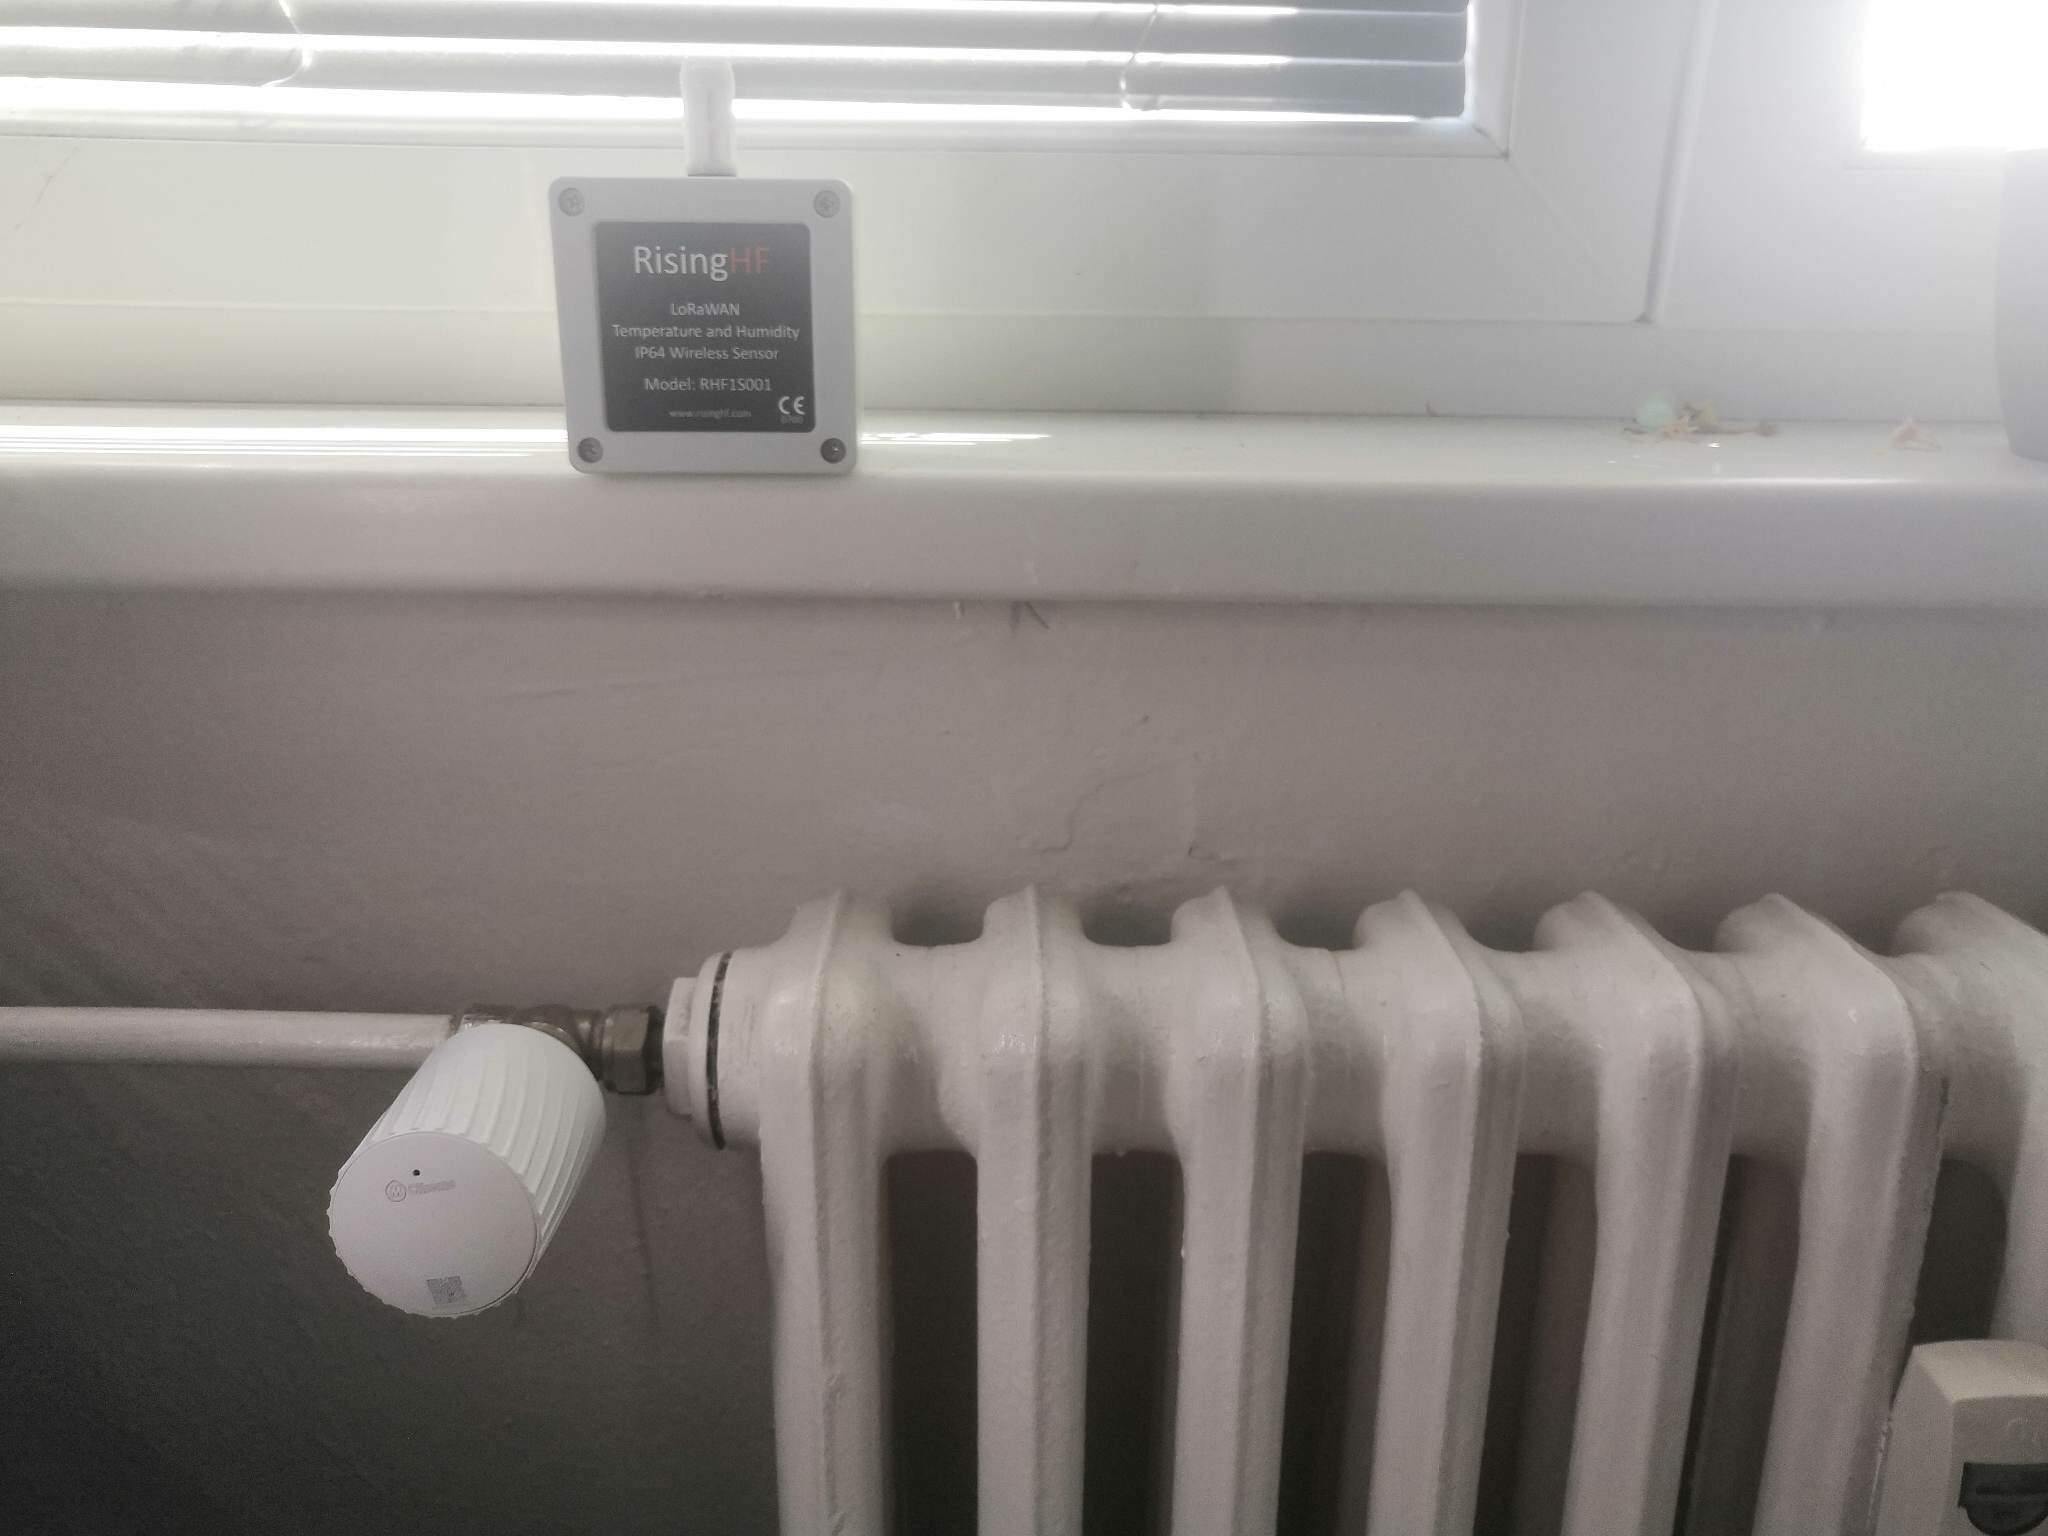
\includegraphics[width=\textwidth]{obrazky-figures/dev_picture_1.jpg}
    \end{subfigure}
    \begin{subfigure}[b]{0.45\textwidth}
        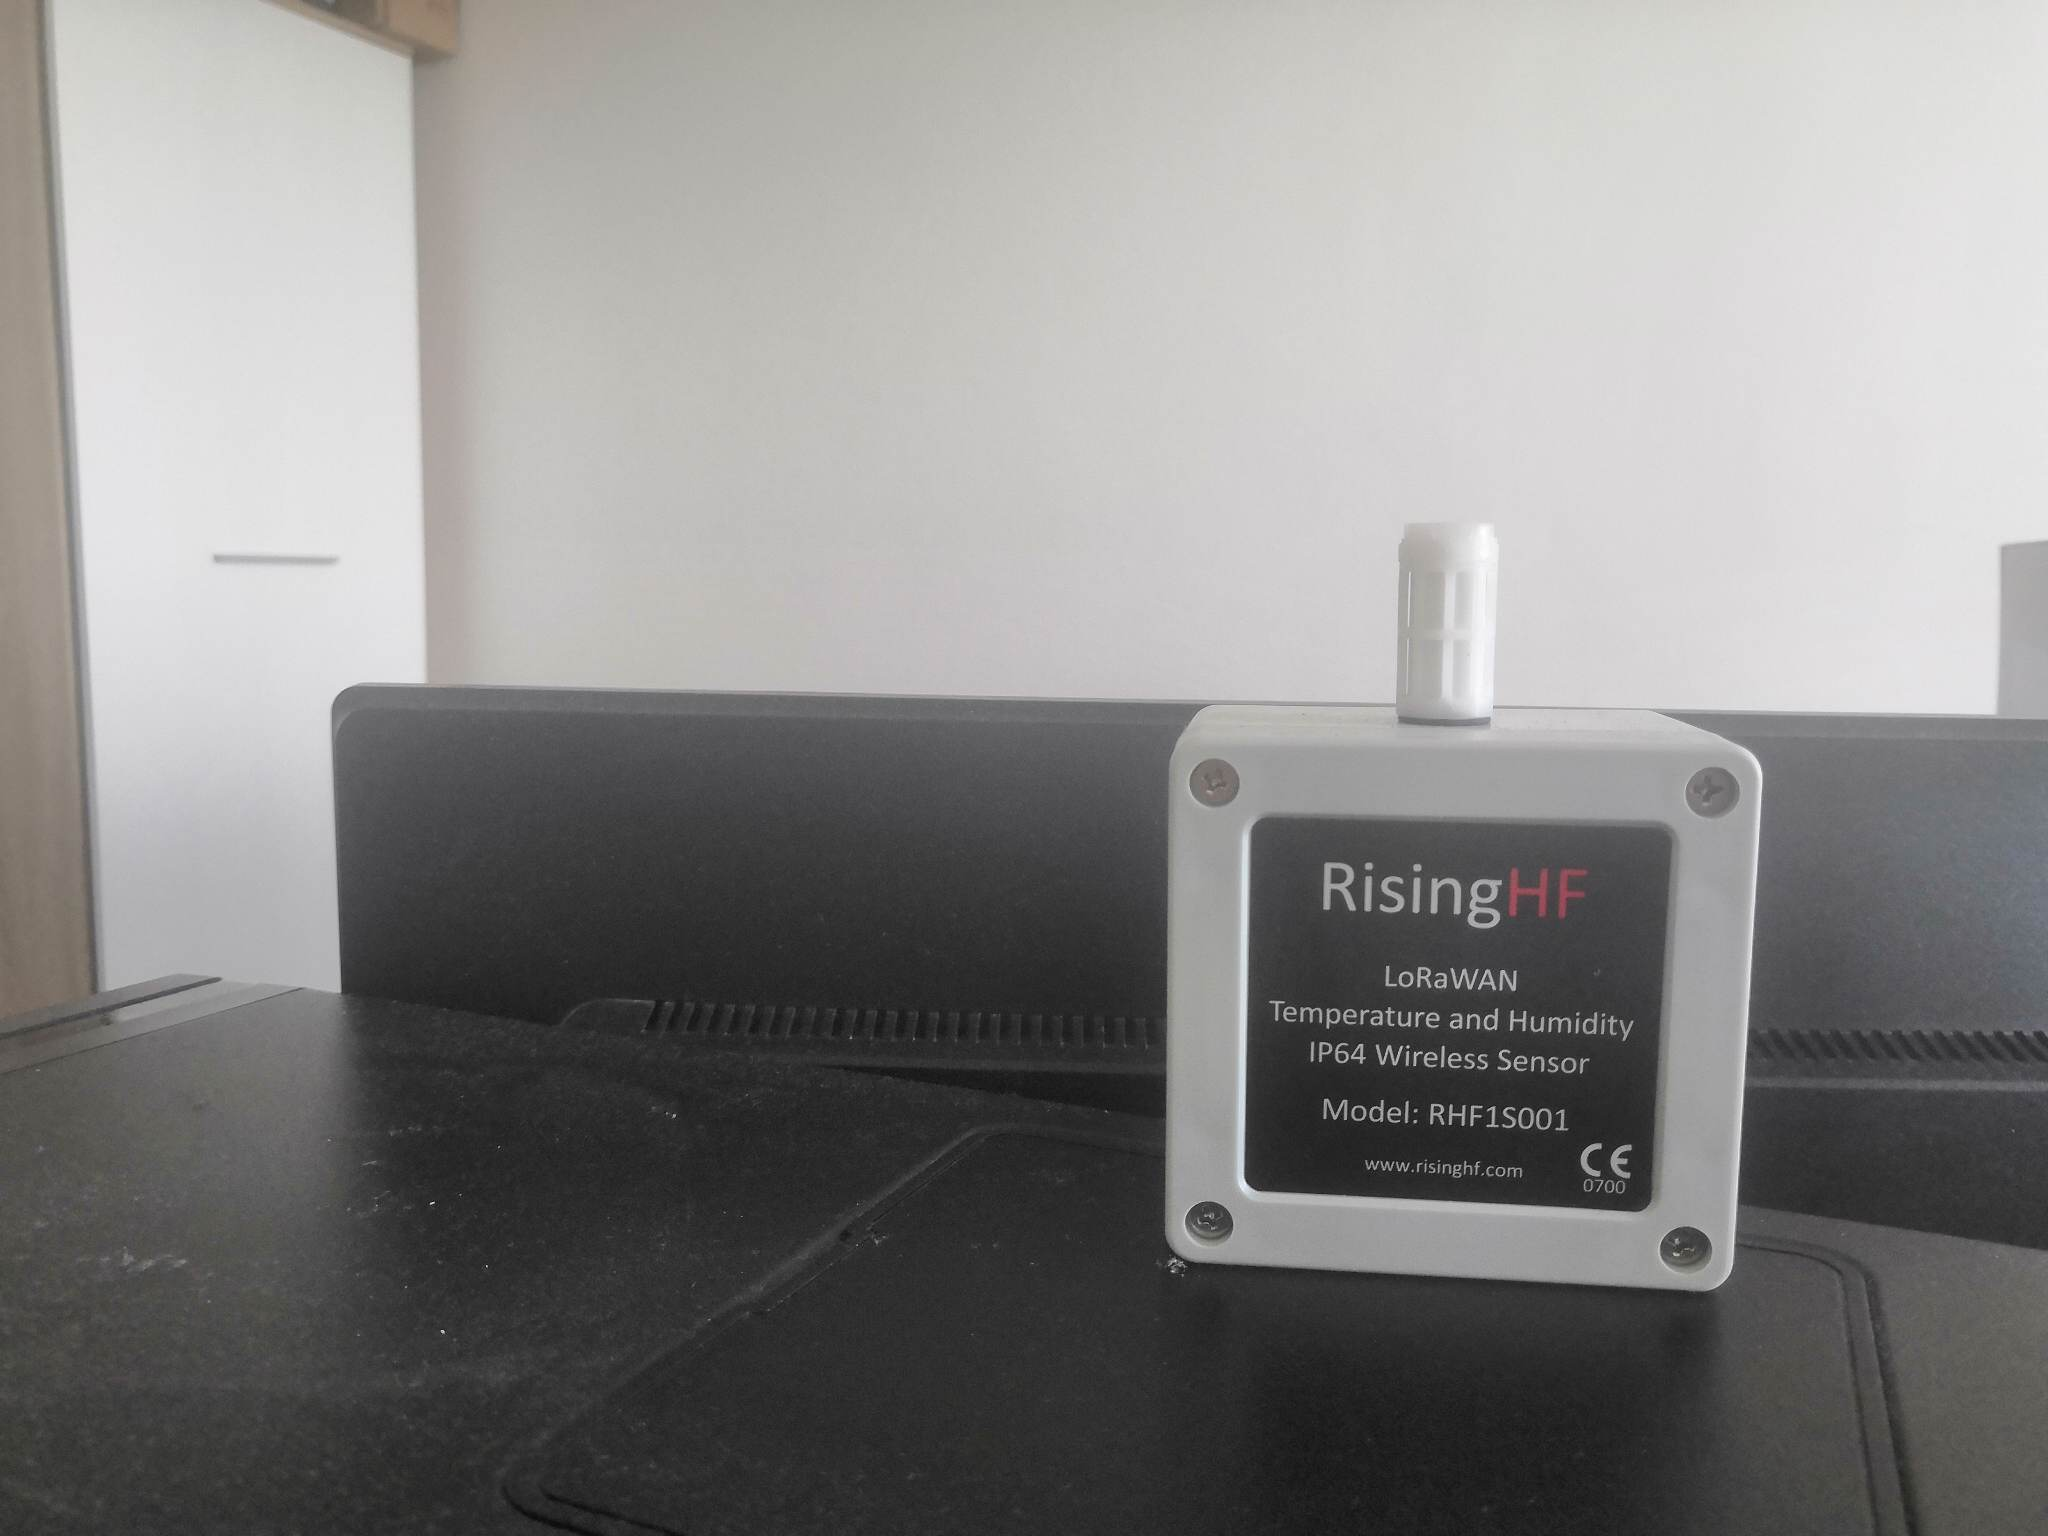
\includegraphics[width=\textwidth]{obrazky-figures/dev_picture_2.jpg}
    \end{subfigure}
    \caption{Zariadenia monitorujúce a ovládajúce teplotu miestnosti.}
    \label{fig:test_device}
\end{figure}

\begin{figure}[H]
    \centering
    \begin{subfigure}[b]{\textwidth}
        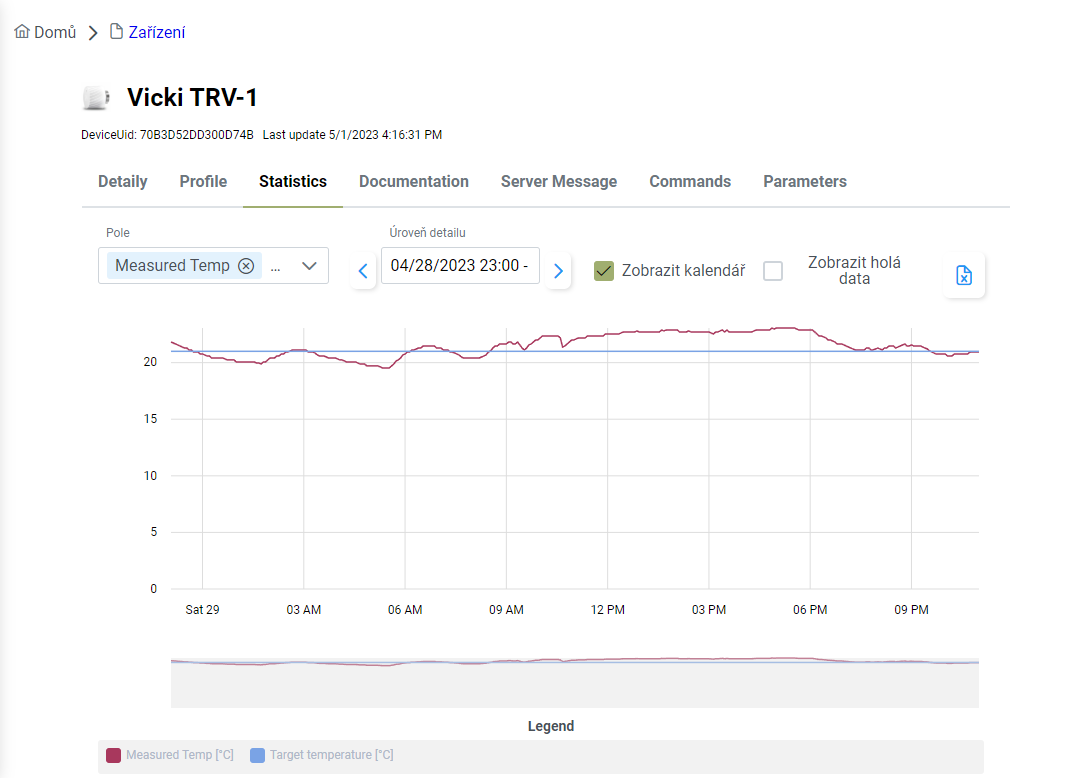
\includegraphics[width=\textwidth]{obrazky-figures/iTempStatisticTemp.png}
    \end{subfigure}
    \begin{subfigure}[b]{\textwidth}
        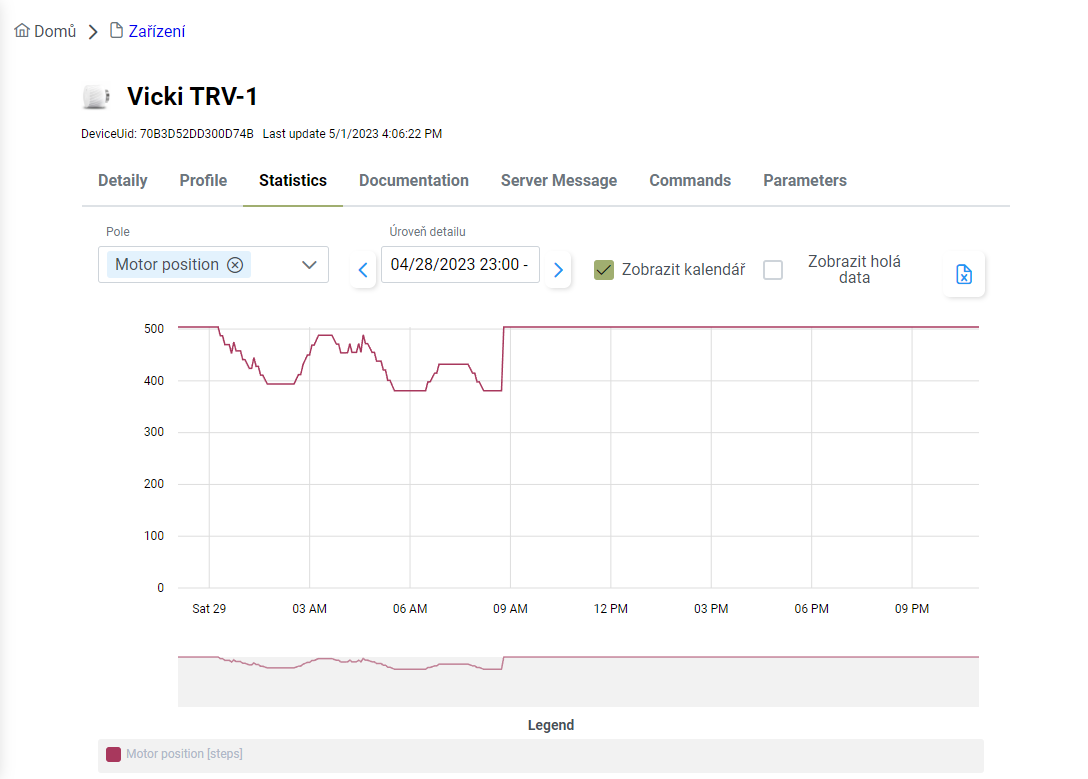
\includegraphics[width=\textwidth]{obrazky-figures/iTempStatisticPosition.png}
    \end{subfigure}
    \caption{Štatistiky z aplikácie iTemp.}
    \label{fig:test_itempStat}
\end{figure}

\begin{figure}[H]
    \centering
    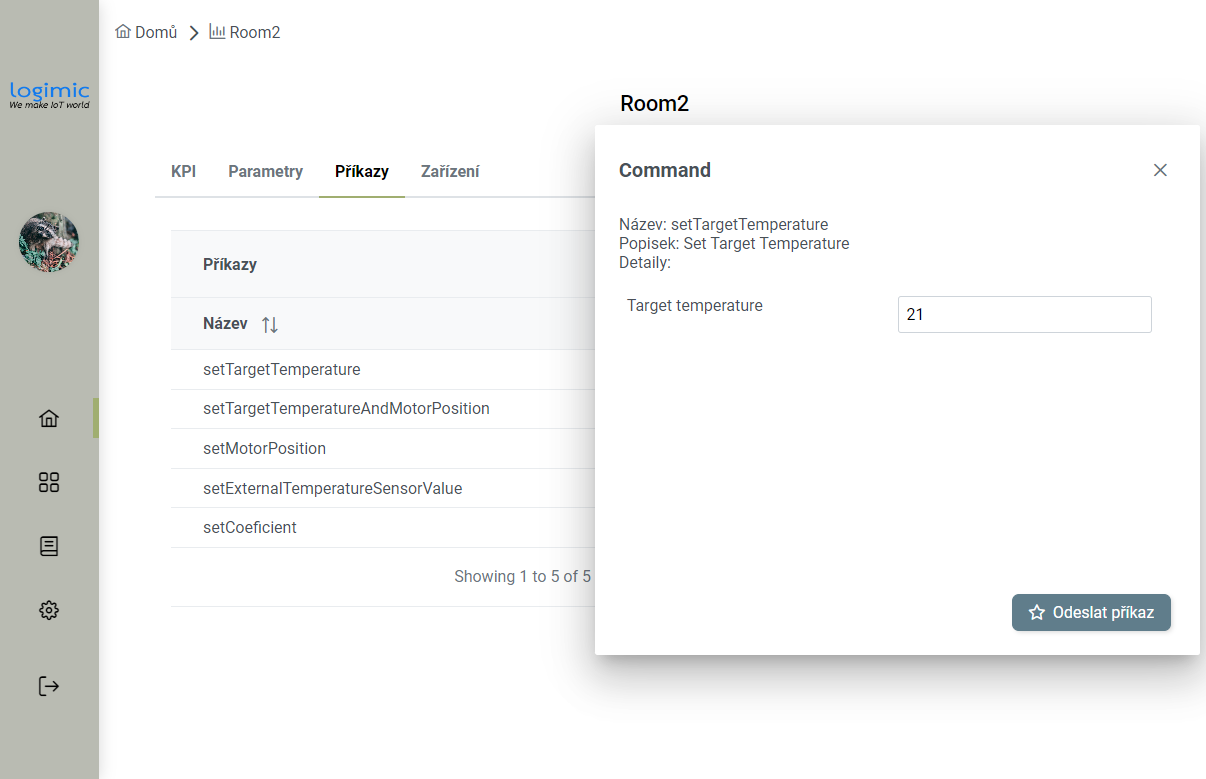
\includegraphics[width=0.9\textwidth]{obrazky-figures/setTarget.png}
    \caption{Nastavenie požadovanej teploty.}
    \label{fig:test_setTarget}
\end{figure}



\begin{figure}[H]
    \centering
    \includesvg[inkscapelatex=false,width=0.9\textwidth]{obrazky-figures/statisticGraph.svg}
    \caption{Graf vývoja teplôt a pozície motora v čase s chybou.}
    \label{fig:statisticGraph}
\end{figure}

\begin{figure}[H]
    \centering
    \includesvg[inkscapelatex=false,width=\textwidth]{obrazky-figures/statisticGraph01.svg}
    \caption{Graf vývoja teplôt a pozície motora v čase.}
    \label{fig:statisticGraph01}
\end{figure}